%&pdflatex
% This is a template for Ph.D. dissertations in the UCI format.
%
% All fonts, including those for sub- and superscripts, must be 10
% points or larger.  Recommended sizes are 14-point for chapter
% headings, 12-point for the main body of text and figure/table
% titles, and 10-point for footnotes, sub- and super-scripts, and text
% in figures and tables.
%
% Notes: Add short title to figures, sections, via square brackets,
% e.g. \section[short]{long}.
%
\documentclass[12pt,fleqn]{ucithesis}

% A few common packages
\usepackage{amsmath}
\usepackage{amsthm}
\usepackage{array}
\usepackage{graphicx}
%\usepackage{siunitx}
%\usepackage{natbib}
\usepackage{relsize}
\usepackage{upgreek}

% Some other useful packages
\usepackage{caption}
\usepackage{subcaption}  % \begin{subfigure}...\end{subfigure} within figure
\usepackage{multirow}
\usepackage{tabularx}
\usepackage{notoccite} % fixes citation numbering when captions have citations
\usepackage{achemso}
\usepackage{chapterbib} % allows separate bib for each chapter(?)

% plainpages=false fixes the "duplicate ignored" error with page counters
% Set pdfborder to 0 0 0 to disable colored borders around PDF hyperlinks
\usepackage[plainpages=false,pdfborder={0 0 0}]{hyperref}

% Uncomment the following two lines to use the algorithm package,
% which provides an algorithm environment similar to figure and table
% ("\begin{algorithm}...\end{algorithm}"). A list of algorithms will
% automatically be added in the preliminary pages. Note that you
% probably want a package for the actual code to go with this (e.g.,
% algorithmic).
%\usepackage{algorithm}
%\renewcommand{\listalgorithmname}{\protect\centering\protect\Large LIST OF ALGORITHMS}

% Uncomment the following line to enable Unicode support. This will allow you
% to enter non-ASCII characters (such as accented characters) directly without
% having to use LaTeX's awkward escape syntax (e.g., \'{e})
% note: You may have to install the ucs.sty package for this to work. See:
% http://www.unruh.de/DniQ/latex/unicode/
\usepackage[utf8x]{inputenc}

% Uncomment the following to avoid "widowing", where page breaks cause
% single lines of paragraphs to float onto the next page (this is not
% a UCI requirement but more of an aesthetic choice).
\widowpenalty=10000
\clubpenalty=10000

% Modify or extend these at will.
\newtheorem{theorem}{\textsc{Theorem}}[chapter]
\newtheorem{definition}{\textsc{Definition}}[chapter]
\newtheorem{example}{\textsc{Example}}[chapter]

% Macros for title, author, abstract, etc.
\thesistitle{Parallel screening for rapid identification of orthogonal bioluminescent tools}

\degreename{Doctor of Philosophy}

% Use the wording given in the official list of degrees awarded by UCI:
% http://www.rgs.uci.edu/grad/academic/degrees_offered.htm
\degreefield{Organic Chemistry}

% Your name as it appears on official UCI records.
\authorname{Colin Michael Rathbun}

% Use the full name of each committee member.
\committeechair{Associate Professor Jennifer Prescher}
\othercommitteemembers
{
  Professor Scott Rychnovsky\\
  Professor Chris Vanderwal
}

\degreeyear{2012}

\copyrightdeclaration
{
  {\copyright} {\Degreeyear} \Authorname
}

% If you have previously published parts of your manuscript, you must list the
% copyright holders; see Section 3.2 of the UCI Thesis and Dissertation Manual.
% Otherwise, this section may be omitted.
% \prepublishedcopyrightdeclaration
% {
% 	Chapter 4 {\copyright} 2003 Springer-Verlag \\
% 	Portion of Chapter 5 {\copyright} 1999 John Wiley \& Sons, Inc. \\
% 	All other materials {\copyright} {\Degreeyear} \Authorname
% }

% The dedication page is optional.
\dedications
{
  (Optional dedication page)
  xxx
  To ...
}

\acknowledgments
{
  I would like to thank the National Science Foundation for funding through the Graduate Research Fellowship Program (grant No. DGE-1321846, and Allergan for funding through the Allergan Graduate Fellowship. I would also like to thank the members of the Prescher lab, Bernard Choi, and Bruce Tromberg, for very helpful discussions. xxx

  You also need to acknowledge any publishers of your previous
  work who have given you permission to incorporate that work
  into your dissertation. See Section 3.2 of the UCI Thesis and
  Dissertation Manual.)
}


% Some custom commands for your list of publications and software.
\newcommand{\mypubentry}[3]{
  \begin{tabular*}{1\textwidth}{@{\extracolsep{\fill}}p{4.5in}r}
    \textbf{#1} & \textbf{#2} \\
    \multicolumn{2}{@{\extracolsep{\fill}}p{.95\textwidth}}{#3}\vspace{6pt} \\
  \end{tabular*}
}
\newcommand{\mysoftentry}[3]{
  \begin{tabular*}{1\textwidth}{@{\extracolsep{\fill}}lr}
    \textbf{#1} & \url{#2} \\
    \multicolumn{2}{@{\extracolsep{\fill}}p{.95\textwidth}}
    {\emph{#3}}\vspace{-6pt} \\
  \end{tabular*}
}

% Include, at minimum, a listing of your degrees and educational
% achievements with dates and the school where the degrees were
% earned. This should include the degree currently being
% attained. Other than that it's mostly up to you what to include here
% and how to format it, below is just an example.
\curriculumvitae
{

\textbf{EDUCATION}

  \begin{tabular*}{1\textwidth}{@{\extracolsep{\fill}}lr}
    \textbf{Doctor of Philosophy in Computer Science} & \textbf{2012} \\
    \vspace{6pt}
    University name & \emph{City, State} \\
    \textbf{Bachelor of Science in Computational Sciences} & \textbf{2007} \\
    \vspace{6pt}
    Another university name & \emph{City, State} \\
  \end{tabular*}

\vspace{12pt}
\textbf{RESEARCH EXPERIENCE}

  \begin{tabular*}{1\textwidth}{@{\extracolsep{\fill}}lr}
    \textbf{Graduate Research Assistant} & \textbf{2007--2012} \\
    \vspace{6pt}
    University of California, Irvine & \emph{Irvine, California} \\
  \end{tabular*}

\vspace{12pt}
\textbf{TEACHING EXPERIENCE}

  \begin{tabular*}{1\textwidth}{@{\extracolsep{\fill}}lr}
    \textbf{Teaching Assistant} & \textbf{2009--2010} \\
    \vspace{6pt}
    University name & \emph{City, State} \\
  \end{tabular*}

\pagebreak

\textbf{REFEREED JOURNAL PUBLICATIONS}

  \mypubentry{Ground-breaking article}{2012}{Journal name}

\vspace{12pt}
\textbf{REFEREED CONFERENCE PUBLICATIONS}

  \mypubentry{Awesome paper}{Jun 2011}{Conference name}
  \mypubentry{Another awesome paper}{Aug 2012}{Conference name}

\vspace{12pt}
\textbf{SOFTWARE}

  \mysoftentry{Magical tool}{http://your.url.here/}
  {C++ algorithm that solves TSP in polynomial time.}

}

% The abstract should not be over 350 words, although that's
% supposedly somewhat of a soft constraint.
\thesisabstract
{
Genetically-encoded fluorescent probes have revolutionized our understanding of biological systems. However, the transition of fluorescent probes in vivo has been hampered by the opacity of tissue and its propensity for autofluorescence. A complementary imaging technology, bioluminescence, does not suffer from these complications because it does not require excitation light. Thus, the technique is exquisitely sensitive—-with the ability to see as few as ten cells in a mouse. Bioluminescence relies on luciferase enzymes that catalyze the oxidation of small-molecule substrates (luciferins), releasing photons of light in the process. Unfortunately, the optimal luciferases for in vivo use rely on the same luciferins, precluding studies of more than one feature at a time.

To address this issue, I developed and analyzed a number of new luciferin probes, and created a selection platform to find mutually orthogonal luciferases and luciferins for multicomponent imaging. In contrast to the spectroscopic resolution of fluorescent tools, these probes were designed to exhibit substrate resolution. Combining luciferin analogs and mutant enzymes, we tested 20 luciferins with 207 luciferases, generating 4,140 enzyme-substrate combinations, and thus a potential for more than 4 million possible sets. Since it would be impractical to evaluate these manually, I derived a mathematical quantification of orthogonality to score each potential pairing. Next, I wrote a supercomputer algorithm to search this dataset for the highest-scoring pairs. The software provided a ranked list of mutually orthogonal enzyme-substrate pairs that were biochemically verified. Resolution was maintained when these probes were moved into mouse models, highlighting the speed and accuracy of my approach.

My most recent work focused on increasing the practicality of these tools for preclinical imaging. The major drawbacks of our approach included temporal resolution and background emission. I addressed these issues by utilizing traditional spectral unmixing algorithms to deconvolute substrate signals mathematically. This enabled sequential imaging of substrates, and the ability to resolve smaller numbers of cells. With a top orthogonal pair I ``unmixed'' gradients of mutant luciferases in bacterial lysate and resolved mixtures of these mutants in mouse tumor models. I am currently applying these techniques to track cells involved in metastasis in mouse models.
}


%%% Local Variables: ***
%%% mode: latex ***
%%% TeX-master: "thesis.tex" ***
%%% End: ***


% Add PDF document info fields
\hypersetup{
	pdftitle={\Thesistitle},
	pdfauthor={\Authorname},
	pdfsubject={\Degreefield},
}

% Uncomment the following to have numbered subsubsections (by default
% numbering goes only to subsections).
%\setcounter{secnumdepth}{4}


% Set this to only select a subset of the includes directives below.
% Very handy to speed up compilation if you're working on a certain
% part of your thesis. It conserves page numbers, references, etc.
% even for non-included files.
\includeonly{chapter2}

% Some customization for figures:
\graphicspath{ {figures/} }
\renewcommand{\floatpagefraction}{.8} % If the fig takes up more than 80% of a page, give it the entire page.

% Some customization for writing easier.
\newcommand{\dluciferin}{{\footnotesize D}-luciferin}
\newcommand{\dluc}{{\footnotesize D}-luc}
\newcommand{\cmpd}[1]{\textbf{#1}}
\renewcommand{\textmu}{$\upmu$}

% Force paragraph indentation?
\setlength{\parindent}{4em}
\setlength{\parskip}{1em}

\begin{document}

% Preliminary pages are always loaded (TOC, CV, etc.)
\preliminarypages

% Include the different components of your thesis, in separate files.
% Using \include allows you to set \includeonly above.
\chapter{Introduction}
Imaging tools enable researchers to ``see" inside tissues and
cells and monitor biological features in real time. While
powerful, most of these probes are confined to monitoring
cellular behaviors at the micro scale, in culture dishes and on
slides. Visualizing cellular behaviors in more authentic environments
requires tools that can function across larger spatial and
time scales.\cite{Porterfield:2015bu} Few probes fit the bill, considering the demands
placed on biocompatibility and sensitivity in whole tissues and
animals. Consequently, basic questions regarding multicellular
interactions in immune function, cell migration, and other
physiological processes remain unanswered.
Bioluminescent probes can address the need for sensitive
imaging on the macro scale. These tools derive from naturally
glowing organisms (e.g., fireflies). All bioluminescent species
produce light via the luciferase-catalyzed oxidation of a small
molecule luciferin. Luciferase enzymes and luciferin substrates
can be imported into diverse cell types and engineered to
report on biological processes.2 The bioluminescent signal is
inherently weak (especially when compared to conventional
fluorescence imaging), but there is virtually no background
emission. Fluorescence imaging, by contrast, relies on light-based
excitation sources that can induce tissue autofluorescence
and result in poor signal-to-noise ratios. Because bioluminescence
requires no excitation light, it can enable
exquisitely sensitive imaging even in heterogeneous tissues. In
fact, bioluminescent probes can be preferred to fluorescent
tools for long-term cell tracking in rodent and other opaque
models. One can serially image luciferase reporters without
detriment to organisms and without knowing ?when and
where? to apply excitation light.
The versatility of bioluminescence has enabled a broad range
of biological studies, although limitations persist.2 This imaging
modality has long been plagued by a lack of bright, easily
distinguishable probes and poor spatial resolution. However,
advances in luciferin chemistry and luciferase engineering have
begun to address these issues. This perspective will highlight
recent achievements in developing new and improved imaging
tools. Collectively, the bioluminescent probes are addressing
long-standing voids in imaging capabilities and are being
applied to ?seeing? biology beyond the culture dish.
\section{Bioluminescence Basics}
Millions of luciferases exist in the natural world, but
phylogenetically related enzymes use the same luciferin.3 The
identities of such luciferins remain exceedingly difficult to
characterize, and of those reported to date, only two have found
routine application in mammalian cell imaging.2 The first, Dluciferin
(Figure 1A), is used by the firefly and a number of
other terrestrial organisms to produce light. The second,
coelenterazine (Figure 1B), is a molecule found in bioluminescent
sea creatures, including the sea pansy Renilla
reniformis and deep-sea copepods Gaussia princeps and
Oplophorus gracilirostris. 

\begin{figure}
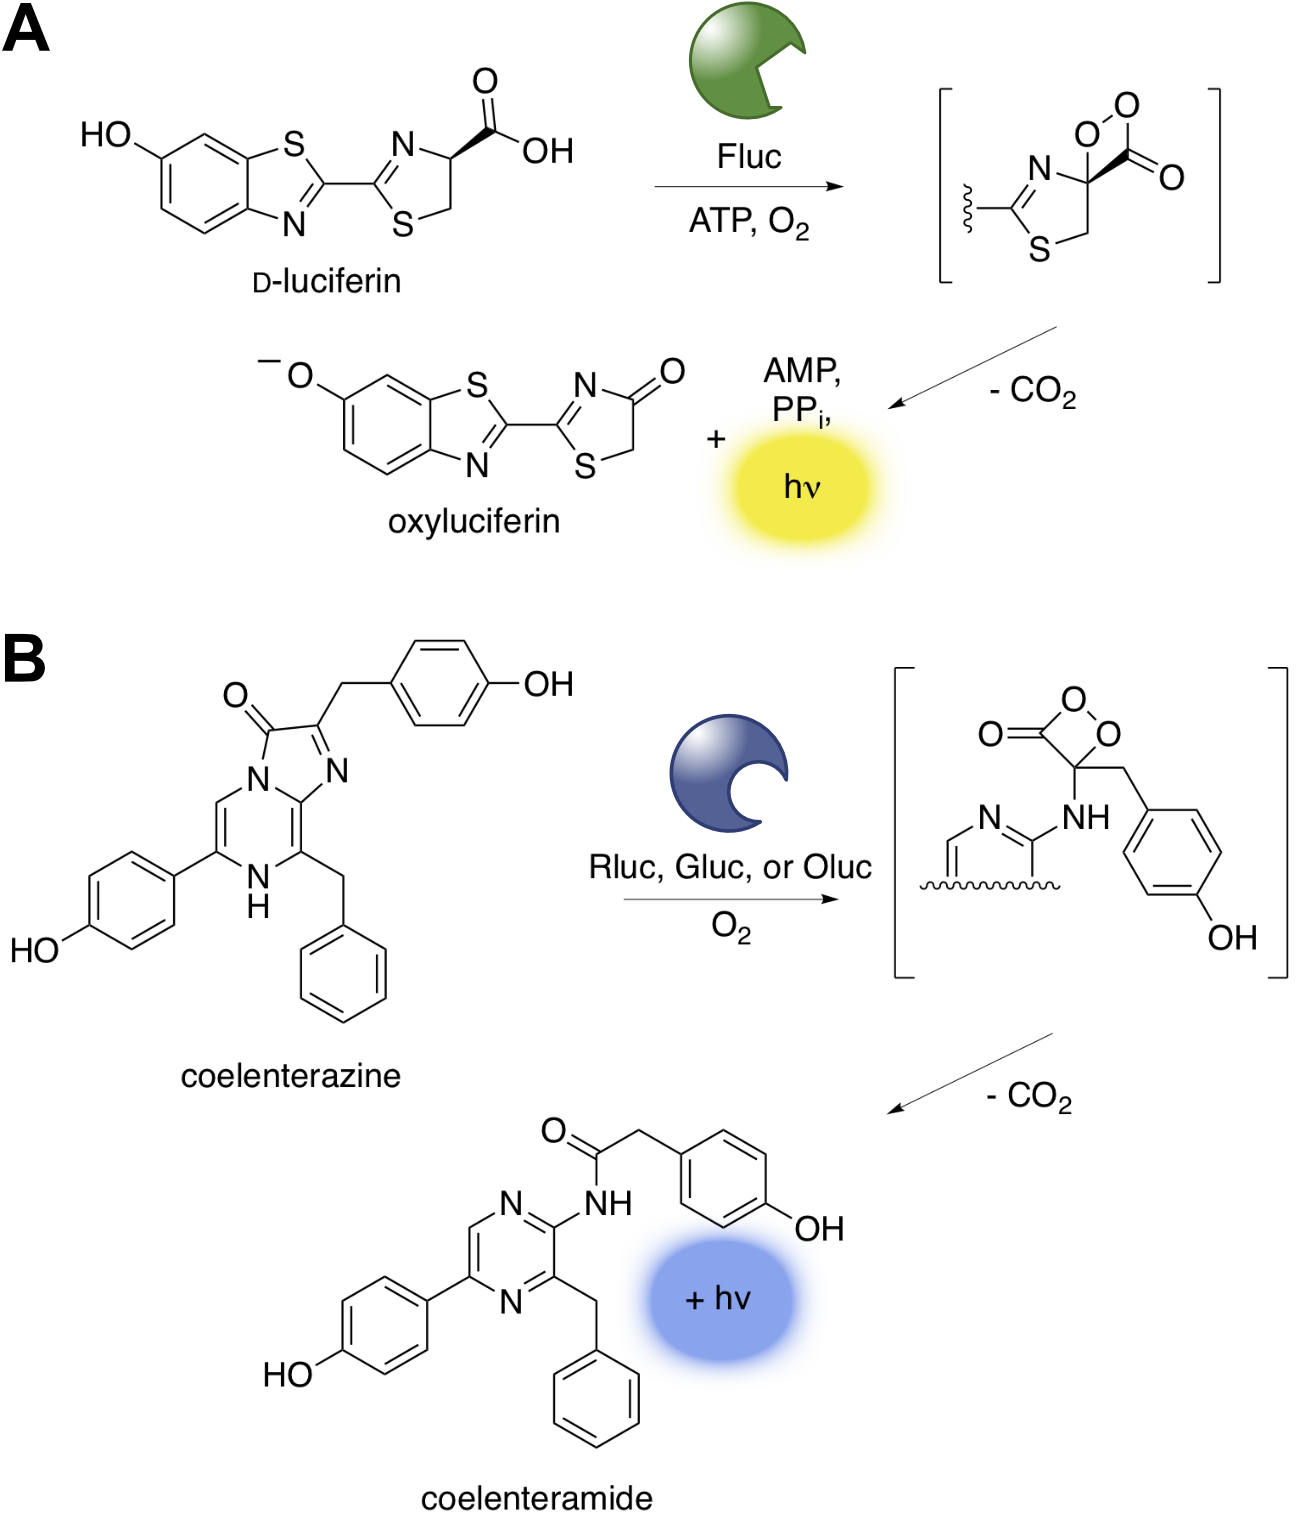
\includegraphics{chapter1/figure1}
\caption{Popular luciferase?luciferin pairs for cellular imaging. (A) DLuciferin
is oxidized by firefly luciferase (Fluc) to produce oxyluciferin
and a photon of light. (B) Coelenterazine is oxidized by a variety of
marine luciferases, including Renilla luciferase (Rluc), Gaussia
luciferase (Gluc), and Oplophorus luciferase (Oluc). These luciferases,
unlike Fluc, require only oxygen as a cofactor in the light-emitting
reaction.}
  \label{fig:luc_oxidation}
\end{figure}

Despite their distinct chemical
structures, D-luciferin and coelenterazine use a similar
mechanism for light production: the cognate luciferases oxidize
the small molecules to generate excited state oxyluciferins;
relaxation of these molecules to the ground state results in
photon emission (Figure 1).
The color of light released is primarily dictated by the small
molecule luciferin. In the case of D-luciferin, the aromatic core
is sufficiently extended to provide yellow-green (?560 nm)
light. For coelenterazine, the ? system of the putative emitter is
shorter, resulting in blue wavelengths (?475 nm) of emission.
The luciferase environment can further modulate bioluminescent
color. Thus, enzymes that use the exact same substrate can
emit different wavelengths. In some cases, the emission spectra
are sufficiently resolved to enable multicolor imaging.4
Discriminating among related luciferases in vivo, though,
remains difficult because of their broad emission spectra and
the strong absorption of <650 nm light.5
\section{Building better bioluminescent tools}
Luciferases and luciferins have been used for decades to image
biomolecules, gene expression, and even whole cells, but the
most popular probes are not without limitation.2 The poor
tissue penetrance of many luciferins has historically precluded
sensitive imaging in hard-to-access tissues (e.g., brain).
Additionally, only a limited ?palette? of bioluminescent probes
exists, hindering efforts to visualize multicellular or other
multicomponent processes. Chemical and biological approaches
are beginning to address the need for improved and
more diverse collections of bioluminescent probes.
Streamlined and Scalable Luciferin Syntheses. Most
bioluminescence imaging studies require an exogenously
delivered luciferin. For in vivo work, the doses can range
between 1 and 5 mg per mouse per imaging point. Thus,
large--and often prohibitively expensive--quantities of luciferin
are required for animal studies. Accessing luciferins in bulk
has been a historic challenge. The chemical complexity of Dluciferin
and coelenterazine has also frustrated efforts to rapidly
diversify these scaffolds to produce new analogues.
In recent years, improved methods for producing luciferins
have been reported. In the case of D-luciferin, we developed a
streamlined method for accessing the requisite benzothiazole
core using Appel?s salt and modern C?H activation (Figure
2).6 This approach improved the yield and generalizability of
the synthesis, eliminating the need for multiple functional
group conversions used in previous routes. The strategy has
enabled multigram syntheses of D-luciferin and has proven to
be quite modular. In fact, we and others have used this
chemistry to produce more than 30 distinct analogues.7 Many
of these scaffolds also comprise key functional handles for latestage
diversification (Figure 2). Efforts to expediently
synthesize amino luciferins8 and related analogues9 are similarly
facilitating more widespread use of bioluminescent tools.
Improved methods for accessing coelenterazine analogues
are also advancing imaging studies. Historically, coelenterazine
synthesis relied on condensation of glyoxal derivatives with
strong acid and elevated temperatures. These conditions are
incompatible with a diverse array of desired analogues. Kirkland
and colleagues identified milder conditions to access the
coelenterazine core via Horner?Wadsworth?Emmons olefination.10
The method proved to be both scalable and generalizable,
providing a range of useful analogues. Recent advances
in cross-coupling methodology are similarly enabling access to
diverse coelenterazine architectures.11
Brighter and More Colorful Probes. Bioluminescence
imaging to date has been largely confined to imaging one or
two colors at a time. Accessing a full spectrum of emitters has
been a long-standing goal, with obvious parallels to
fluorescence imaging. Early efforts to modulate color and
brightness primarily focused on the luciferase enzyme.2 Recent
years, though, have seen a shift in focus to modulating the small
molecule (Figure 3).
Because the structure of the luciferin emitter influences
bioluminescent output, methods for modulating color and
intensity often parallel those in small molecule fluorophore
development. For example, rigidifying the aromatic core can
provide improved ?push?pull? chromophores and enhanced
light emission. Miller and co-workers applied this strategy to Dluciferin,
replacing the rotationally flexible 6? electron-donating
group with a conformationally locked amine.12 This configuration
enabled enhanced donation of electrons to the luciferin
core and more robust, red-shifted emission compared to that of
related probes. Moreover, many of the cyclic luciferin (CycLuc)
scaffolds were viable substrates for Fluc, highlighting the
promiscuity of the enzyme.
Fluc can also process luciferin analogues with extended
aromatic cores and modified heteroatoms, providing additional
avenues for wavelength alteration.6,7,13 ?-Extended chromophores
typically emit red-shifted light emission.14 In the case of
the vinyl-extended luciferins (Figure 3), the shift was >100 nm.
It should be noted, though, that these and other extended
analogues are often poorly processed by Fluc itself; red-shifted
emission comes at the expense of enzyme turnover and thus
total photon output.
Parallel developments in coelenterazine synthesis have
provided scaffolds that emit different colors of light. Redshifted
probes are particularly desirable for imaging with Rluc
and Gluc in vivo, as the ?normal? blue emission with these
enzymes is strongly absorbed by blood.5 Inouye and colleagues
recently developed a streamlined synthesis of a conformationally
locked coelenterazine for improved imaging.11 Others have
explored luminophores with extended ? conjugation to achieve
more tissue-penetrant wavelengths of light.15,16
Bioluminescent color and photon output can also be
drastically modulated via bioluminescent resonance energy
transfer (BRET). A recent fusion of NanoLuc (an optimized
mutant luciferase, discussed below) to CyOFP1 [dubbed
Antares (Figure 4A)] resulted in an emission shift of 114 nm
(Figure 4B).17 Antares is one of the most red-shifted BRET
pairs reported to date, enabling enhanced deep-tissue imaging
in vivo (Figure 4C). In related work, Nagai and colleagues
linked a mutant Renilla luciferase to Venus, a version of yellow
fluorescent protein.18 Unexpectedly, this construct (dubbed
Nanolantern) produced 6-fold more photons than the
luciferase alone and shifted emission into the yellow-green
region (530 nm). Additional Nanolantern colors have been
described.4 Collectively, these and other BRET probes are
enabling sensitive imaging of many biological processes,
including membrane voltage19 and gene expression.20
In Vivo Improvements. Luciferins can access most tissues,
but their distribution and cell permeability are suboptimal and
not uniform.22 Chemical tinkering and med-chem optimization
can improve the bioavailabilities of the substrates. For example,
many of the CycLuc scaffolds that comprise more lipophilic
amino modifications (vs ?OH groups) exhibit improved tissue
penetrance in vivo.23 Far less compound is required for a given
imaging session compared to native luciferins. Further
amidation of a CycLuc probe enhanced its transport across
the blood?brain barrier (Figure 5).21 Once the probe is in the
brain, the amide bond can be cleaved by endogenous fatty acid
amide hydrolase (strongly expressed in brain tissue), releasing a
functional luciferin.
\section{Luciferase-luciferin pairs for multicellular imaging}
Many improvements to the luciferin small molecules noted
above came at the expense of luciferase turnover (and thus light
output). Consequently, recent efforts to build improved
bioluminescence tools have focused on identifying new
substrates and enzymes in parallel. One source of new
luciferase?luciferin pairs is nature itself. Bioluminescent
organisms (and potentially new luciferase?luciferin pairs) are
continually being described,24 though the need for optimized
probes far outpaces their discovery. Others have turned to
engineering existing luciferases to better use chemically
modified luciferins. In one example, Miller identified mutant
luciferases that can more readily process CycLuc derivatives.
These analogues were previously demonstrated to be viable
substrates for Fluc, although oxyluciferin products inhibited the
reaction. Substrate inhibition was relieved and long-lived light
emission restored with mutant enzymes.25 The authors later
identified a mutant that preferred a luciferin analogue over Dluciferin,
setting the stage for developing substrate-responsive
enzymes.26 Further work by the Miller group revealed ?latent?
luciferase activity in a fatty acyl-CoA synthetase from the
fruitfly.27 Interestingly, this enzyme did not emit light with Dluciferin?it
was able to use only a CycLuc substrate?opening
the door to pairing unnatural luciferin analogues with
evolutionary relatives of luciferase.
Another engineered bioluminescent enzyme that has seen
widespread adoption in recent years is NanoLuc, a derivative of
Oplophorus luciferase (Oluc).28 Early work in this area was
motivated by the need for improved coelenterazines (molecules
prone to autoxidation and exhibiting poor tissue penetrance)
and Oluc subunits (enzyme fragments prone to instability).
Seeking a brighter and more stable luciferin, Wood and
colleagues replaced the electron-rich phenols of coelenterazine
with phenyl and furan groups. The resulting molecule
[furimazine (Figure 3)] was more stable in media and lysate
and less susceptible to nonspecific oxidation. Directed
evolution was used to select an enzyme that could readily
catalyze light emission from the designer luciferin. The
?winning? mutant (NanoLuc) contained a total of 16
mutations, an impressive number for a 16 kDa protein.
NanoLuc exhibits a high turnover rate with furimazine,
providing robust signal output. Such high photon flux values
are enabling sensitive imaging in complex tissue samples, even
point-of-care diagnostics with simple cell phone cameras.29 We
anticipate that the popularity of the NanoLuc?furimazine pair
will continue to surge in the near term.
Tandem modification of bioluminescent enzymes and
substrates is also enabling multicomponent bioluminescence
imaging. In contrast to in vitro assays, imaging in vivo often
precludes spectroscopic resolution of colored probes. Blood
and tissue restrict the passage of wavelengths shorter than red,5
and bioluminescence spectra are broad,31 necessitating an
alternative approach. Substrate resolution is one such strategy
(Figure 6A). This approach requires multiple selective,
mutually orthogonal luciferin?luciferase pairs. These pairs
produce light together but will not react with other mutants or
enzymes. Orthogonal pairs already exist in nature (e.g., firefly
and marine luciferases, along with their requisite substrates),
and many have been adapted for dual-imaging studies.
To expand and expedite the search for orthogonal pairs,30 we
turned to producing non-natural analogues and enzymes. We
synthesized a panel of luciferins, with additional steric bulk at
the 4? and 7? positions (Figure 6B). We screened these
analogues against libraries of luciferase mutants to produce
more than 3000 potential pairings. To find substrate-resolved
hits in this milieu, we mined the data with a computer
algorithm. This strategy revealed two enzymes that exhibited
substrate resolution with two compounds (one 4? and one 7?).
This pair proved to be successful in mammalian cells, as well,
demonstrating the robust nature of our screening methodology
(Figure 6C). In an analogous approach, Kim and colleagues
recently reported substrate-resolved bioluminescence imaging
with coelenterazine analogues.32
\section{Bioluminescent reporters for cell--cell interactions}
A second challenge being addressed by improved bioluminescent
tools is monitoring cellular interactions in vivo.
Conventional bioluminescence imaging can detect small
numbers of cells, but historically has lacked the spatial
resolution to precisely pinpoint their locations or interactions
in whole organisms. Target recognition and cell?cell contacts
are crucial to numerous physiological processes, including
neurotransmission, immune function, and cell migration, so
methods to globally assay such interactions are necessary.
The development of tools that report on cell?cell contacts
has been inspired by classic methods for reporting on
biomolecule activities and interactions. For example, caged
probes have been used widely to report on small molecule
analytes in cells. We and others33 have shown that such cages
can be repurposed to image interactions between cells (Figure
7A). In a recent example, a ?dark? luciferin comprising a 6?-
nitro group (Luntr) was used as the cage.34 This probe could
be reduced by one group of cells (expressing nitroreductase)
and used by a neighboring group of cells expressing luciferase.
Light emission was strongest in areas of cellular contact.
Nitroreductase is not expressed endogenously in mammalian
cells, making this technology ripe for in vivo applications where
high spatial sensitivity is required.
A second class of cell contact sensors uses split reporters,
originally developed to image protein?protein interactions
(Figure 7B). We expanded on this concept to generate split
reporters of cell proximity using Gaussia luciferase (Gluc), a
secreted protein that functions in the extracellular space. Split
fragments of Gluc were fused to leucine zippers Fos and Jun to
drive complementation. The N-terminal half was expressed in
one cell population and the C-terminal half in another. Light
emission in this case tracked with distance between the cell
populations (Figure 7C).
\section{Bioluminescent reporters for analyte detection in vivo}
Bioluminescence has long been exploited for detecting enzyme
activities and low-abundance metabolites. The majority of these
studies, though, have been limited to ex vivo analyses with
cultured cells or excised tissues. Continued advances in
bioluminescence technology are enabling new probes to be
applied as biosensors in vivo.36,37 In a recent example, Chang
and colleagues developed a copper ion sensor for imaging in
mice. The probe comprised a caged luciferin, with a bulky
chelator group (i.e., the ?cage?) attached to the 6? position of Dluciferin.
The sterically encumbered molecule was poorly
utilized by luciferase. Upon removal of the cage by copper-
(I)-dependent oxidative cleavage, a viable luciferin was liberated
and available for light emission. Photon production could thus
be correlated to copper ion levels. The caged probe was
ultimately used for analyte imaging in mouse models of fatty
liver disease.36
\section{Conclusions and future directions}
Bioluminescence has historically lagged behind fluorescence
imaging in terms of the breadth and diversity of available tools.
Recent advances in luciferin chemistry and luciferase engineering,
though, are beginning to fill this gap. New synthetic
methods are providing novel luciferin architectures for
improved imaging. Engineered luciferases are enabling the
sensitive detection of cells and other analytes in vivo.
Combinations of designer substrates and mutant enzymes are
furthering the range of potential applications. It is now possible
to image multicellular features in live animals, visualize cells in
difficult-to-access tissues (e.g., brain tissue), and selectively
illuminate cell?cell interactions. Moving forward, we anticipate
continued advances in red-shifted probes, tandem luciferase?
luciferin engineering, and sensors for cellular metabolites.
These tools will influence how researchers conduct experiments
involving multiple cell types and molecular features beyond the
culture dish. Additionally, like other useful imaging agents, the
tools will likely facilitate discoveries in a diverse range of fields.

%%% Local Variables: ***
%%% mode: latex ***
%%% TeX-master: "thesis.tex" ***
%%% End: ***

\chapter{Orthogonal Luciferase−Luciferin Pairs for Bioluminescence Imaging}

\section{Introduction}
Bioluminescence imaging is a popular method for visualizing
cells and other biological features in vivo.\cite{RN26} This technology
relies on enzymes (luciferases) that catalyze the oxidation of
small-molecule substrates (luciferins). The oxidation process is
accompanied by the release of light (Figure \ref{fig:overview}A).
\begin{figure}[htbp]
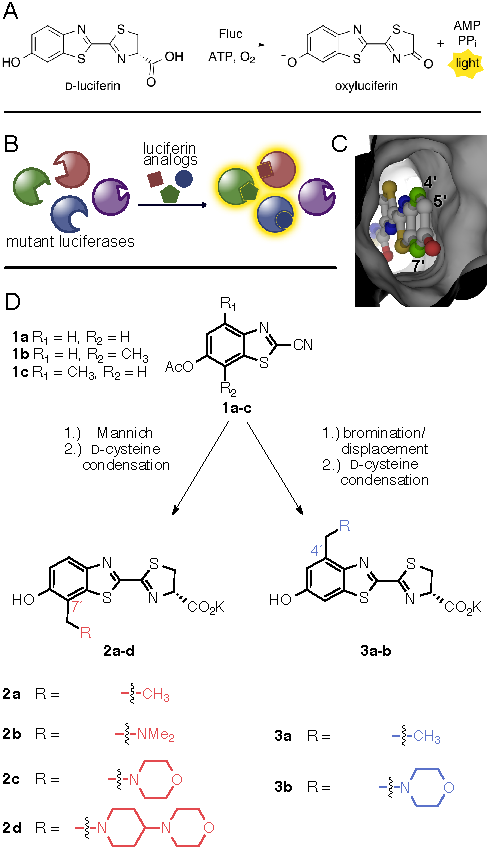
\includegraphics[width=85 mm]{chapter2/fig1}
\centering
\caption[Expanding the bioluminescence toolkit with unique
enzyme−substrate pairs]{Expanding the bioluminescence toolkit with unique
enzyme−substrate pairs. (A) Luciferase-mediated light production
proceeds via an adenylation−oxidation sequence. (B) Strategy to
develop orthogonal luciferase−luciferin pairs via substrate resolution.
Genetically engineered luciferases and chemically modified luciferins
were screened to identify novel partners. Only complementary
enzyme−substrate pairs interact to produce light. (C) Model of \dluciferin{}
bound to firefly luciferase (Fluc). (D) Synthesis of C7′ (left)
and C4′ (right) sterically modified luciferins.}
  \label{fig:overview}
\end{figure}
Since
mammalian cells and tissues do not emit substantial numbers
of photons, bioluminescent light can facilitate sensitive imaging
in these environments.\cite{Prescher:2010dv} Luciferase-labeled cells can also be
imaged repeatedly and noninvasively in a variety of preclinical
models. This broad dynamic range has enabled numerous
studies of fundamental biological processes, including cell
homing and differentiation, proliferation, and cell-to-cell
communication, in physiologically relevant environments.\cite{Badr:2011if}
\par
While versatile, bioluminescence to date has been largely
limited to monitoring one cell type or biological feature at a
time. This is due, in part, to a lack of distinguishable luciferase−
luciferin pairs for in vivo use. The optimal luciferases (from the
insect family) use the same substrate, \dluciferin{}.\cite{RN26,RN101} Thus, they
cannot easily discriminate multiple cell types in a single subject.
Additionally, unlike fluorescent protein technologies, a diverse
suite of accessible bioluminescent probes does not yet exist. To
address this void, \dluciferin{} analogues have been engineered to
emit different colors of light.\cite{RN14,Jathoul:2014do,RN165} However, these substrates are
still utilized by the same luciferases, precluding the distinct
genetic tagging of individual cell types. Insect luciferases have
also been engineered to emit different colors of light with \dluciferin{}.\cite{Branchini:2007fza,Branchini:2007bw,Mezzanotte:2010fq}
The observed emission spectra are not sufficiently
resolved, though, for routine use in complex tissues or animals.
Discriminating among different wavelengths in bioluminescence
(and whole-body optical imaging, in general) is
exceedingly difficult.
\par
Contrasting with these attempts to achieve spectral
resolution, we aimed to obtain distinguishable bioluminescent
probes via substrate resolution. Substrate-resolved bioluminescence
is well precedented in nature, as structurally distinct
luciferase−luciferin pairs have been identified across diverse
phyla.\cite{Haddock:2010cx, Oba:2014cc, Viviani:2002dp} Some of these pairs, including those from the firefly
and Renilla reniformis, have been used extensively.\cite{Paley:2014fl, Badr:2011if, Porterfield:2015bu, Massoud:2007en} Firefly
(Fluc) and Renilla luciferase employ chemically unique
substrates (\dluciferin{} and coelenterazine, respectively), enabling
their tandem application in vivo.\cite{Bhaumik:2002hf, Maguire:2013kb} Coelenterazine is
less ideal for use in these environments, though, owing to its
suboptimal bioavailability and stability.\cite{Paley:2014fl, Pichler:2004ke} Other naturally
occurring luciferases and luciferins can be used in combination
with Fluc/\dluciferin{} or other bioluminescent systems.{Maguire:2013kb, Petushkov:2014ha}
However, most of these native pairs remain poorly characterized
or ill-suited for routine use.
Artificial (i.e., mutant) luciferases can exhibit altered
bioluminescent properties, including tolerance for chemically
modified substrates. Fluc itself has been manipulated to process
analogues of \dluciferin{}.\cite{Evans:2014bv} In elegant work along these lines,
Miller and co-workers prepared a class of non-natural
aminoluciferins that were found to be robust light emitters
with Fluc, but the products inhibited the enzymatic reaction.\cite{Reddy:2010ga}
Product inhibition was relieved using mutated versions of the
enzyme.\cite{Harwood:2011gl} These same mutations also resulted in sharply
reduced emission with \dluciferin{}, providing key precedent for
the development and utilization of orthogonal pairs.\cite{AdamsJr:2016bn} The
mutant enzymes from these studies, though, were less selective
for one analogue over another perhaps due to the structural
similarities between the luciferin scaffolds. Simultaneous enzyme−substrate manipulation has also been applied to
aequorin (a marine photoprotein) and the luciferase from the
deep-sea shrimp Oplophorus gracilirostris.\cite{Rowe:2009bd,Hall:2012cd} In both cases,
altered bioluminescent outputs (e.g., colors and stabilities) were
achieved, but orthogonal substrate usage was not realized.
Here, we report a strategy for the de novo production of
orthogonal luciferase−luciferin pairs. We synthesized a series of
sterically modified luciferins that were poor emitters with Fluc
but intrinsically capable of robust light production. We then
iteratively screened these analogues with libraries of mutant
luciferases and identified substrate-selective enzymes. The
“hits” were also biochemically characterized. Importantly,
when the mutants and analogues were combined, robust light
production was observed when complementary enzyme−
substrate partners interacted. Sequential administration of
substrates enabled unique luciferases to be illuminated (and
thus resolved) within cultured cell models. These tools promise
to enable a variety of multicellular imaging applications.
Importantly, our approach to identifying orthogonal bioluminescence
pairs is also general and should enable rapid
diversification of the bioluminescence toolkit.

\section{Results and Discussion}

\subsection*{Designing and constructing sterically modified luciferins}
To expediently identify orthogonal bioluminescence
tools, we aimed to screen sterically perturbed luciferins
against libraries of mutant luciferases (Figure \ref{fig:overview}B). We used the
Fluc/\dluciferin{} pair as a starting point for several reasons. First,
this duo is the most widely used in biomedical imaging
applications owing to the nontoxicity of the reagents and
bioavailability of the substrate.26,27 Second, the Fluc/\dluciferin{}
reaction releases the highest percentage of tissue-penetrating
light among known bioluminescent families.28 Thus, new
enzymes and substrates based on the firefly pair would be more
applicable to in vivo studies. Third, a wealth of structural and
biochemical information on Fluc could guide our engineering
efforts.13,29−32 Finally, \dluciferin{} derivatives are arguably the
most synthetically tractable luciferin architectures.33,34
Generating an expanded set of bioluminescent tools required
access to diverse luciferin scaffolds. A variety of \dluciferin{}
analogues have been synthesized over the past four
decades,5,7,35−39 and those capable of robust emission with
Fluc harbor common features: an electron-donating group at
the 6′ position, a carboxylate appendage (for adenylation), and
an abstractable proton α to the carboxylate.40,41 Beyond these
requirements, Fluc can tolerate a surprisingly large variety of
modified luciferins,34,36,42 including 6′-amino substituents,20,21,36
alkylated43−45 and acylated46 scaffolds, and even
luciferins with non-natural chromophores.6,47 Crystallographic
analyses have also corroborated these experimental results,
indicating flexibility within the luciferase active site and “space”
to accommodate luciferins with appendages at or near the 6′
position.31,32
Unlike most efforts to produce luciferin analogues reported
to date, we were attracted to the 4′ and 7′ positions of the
luciferin core. These positions lie in close proximity to the Fluc
backbone (Figure \ref{fig:overview}C). Substrates with additional steric bulk at
these sites would likely be occluded from the Fluc active site
and thus good targets for orthogonal probe development: while
poor emitters with the native enzyme, the molecules could
potentially give off light with designer mutants. Indeed,
preliminary docking studies suggested that only analogues
with small (e.g., 2−3 atoms) substituents at C4′ and C7′ could
effectively access the active site.
Generating 4′- and 7′-modified luciferins presented an early
challenge. These positions have been rarely exploited for
analogue development, and no prior syntheses were amenable
to preparing libraries or large quantities of these probes. Rapid,
high-yielding syntheses were essential, as large quantities of
luciferins are required for light emission assays. Fortunately, the
core benzothiazole unit (1a−c) of the desired analogues could
be accessed from a common route (Figure \ref{fig:overview}D) and in
multigram quantities.33,38 From this single intermediate, we
envisioned installing functional handles at C4′ and C7′ to
rapidly assemble a variety of luciferins. We were initially drawn
to an aldehyde group, owing to its ease of diversification under
mild conditions (e.g., reductive amination) and broad
compatibility. Aldehyde installation on 1a was problematic,
though, due to formation of a hydrated hemiacetal.48 To circumvent this issue, we turned to more reactive
iminium ions. These electrophiles can be readily trapped by
electron-rich aromatics in a Mannich-type reaction.49 Toward this end, benzothiazole 1a was modified with a series of tertiary
benzyl amines via in situ iminium formation and coupling
(Figure \ref{fig:overview}D and Schemes S2 and S3). The amino appendages
were selected to enhance the water solubility of the luciferin
core. Importantly, this synthetic approach was modular and
amenable to large-scale (1−10 g) syntheses. “Matched” probes
with steric modifications at C4′ were also prepared (3a,b). A
different synthetic approach was necessary, though, as the 4′
position cannot be selectively targeted with electrophiles
(Figure \ref{fig:overview}D and Scheme S4).

\subsection*{Analyzing bioluminescent light emission with modified luciferins}

With the modified luciferins in hand, we first
evaluated their optical properties with Fluc. All analogues were
competent light emitters and could be processed by the enzyme
(Figures 2A).
\begin{figure}[htbp]
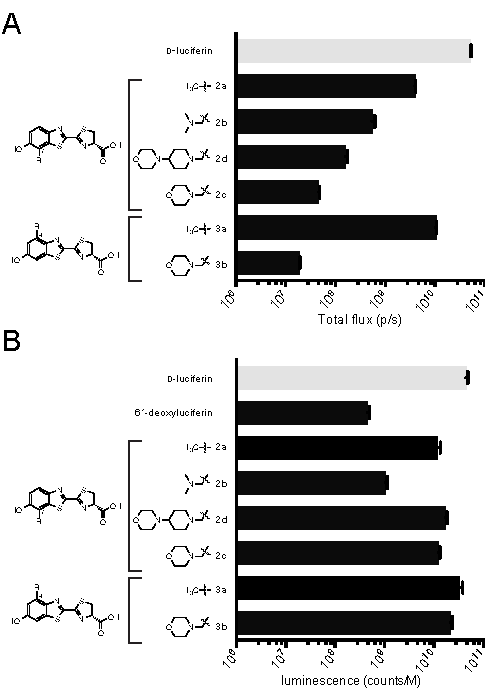
\includegraphics[width=85 mm]{chapter2/fig2}
\centering
\caption[Measuring luciferin light emission]{Measuring luciferin light emission. (A) Bioluminescence
from luciferin analogues (100 μM) incubated with 1 μg of Fluc.
Emission intensities are plotted as total photon flux values on a log
scale. Error bars represent the standard deviation of the mean for n ≥ 3
experiments. (B) Chemiluminescence with luciferin analogues.
Emission intensities are plotted as counts per molar luciferin on a
log scale. Error bars represent the standard error of the mean for n ≥ 3
experiments.}
  \label{fig:chemilum_biolum}
\end{figure}
However, the emission intensities were much weaker than those observed with \dluciferin{}, the native
substrate. Interestingly, the largest analogue (2d) was not the
weakest emitter, suggesting that steric modification alone does
not dictate luciferin utilization. Similar trends in light emission
were observed across a range of physiological pH values
(Scheme S3). Consistent with the observed light outputs, the
measured kinetic constants for all analogues showed reduced performance relative to \dluciferin{} (Table S10). For example,
the measured Km values were ∼100-fold larger than the native
substrate, with the largest analogues (2c and 2d) exhibiting the
lowest relative binding affinities. Despite their large Km values,
2b−d exhibited emission spectra similar to that of \dluciferin{}
(Figures S4 and S5). Only the C4′-modifed analogue 3b
emitted noticeably red-shifted bioluminescent light, likely due
to poor Fluc binding in the excited state32 or the luminophore
being forced into a more polar environment.50,51

\subsection*{Measuring the light-emitting potential of luciferin analogues}

We attributed the weak bioluminescence of the
analogues to poor utilization by Fluc. It was possible, though,
that the luciferins were simply not capable of photon
production upon activation and oxidation in the active site.
For productive bioluminescence, an analogue must be able to
reach an electronic excited state (S1) and relax back to the
ground state with concomitant photon release.52,53 If an
analogue cannot reach S1 or emit efficiently from that state,
reduced photon outputs would be expected. Such molecules
would also be poor candidates for orthogonal probe development.
To ensure that our lead analogues were intrinsically
capable of light emission, we utilized a previously described
chemiluminescence assay.54 This process mimics the enzymatic
reaction itself via formation of an activated ester intermediate,
followed by proton abstraction and subsequent reaction with
molecular oxygen.41,53,55 When analogues 2a−d and 3a,b were
subjected to the assay, robust light emission was observed
(Figure \ref{fig:chemilum_biolum}B). In fact, photon outputs for some of the weakest
bioluminescent emitters (including 2c and 3b) were on par
with \dluciferin{}. A control compound (6′-deoxylucifeirn)
lacking an electron-dense residue on the aromatic ring (a key
feature of luciferins) exhibited only weak levels of emission.
These results provided assurance that while luciferin scaffolds
may be poor substrates for Fluc, they are still capable of photon
production and thus good candidates for orthogonal tool
development.

\subsection*{Evolving substrate-specific luciferases}

Having prepared
candidate orthogonal luciferins, we set out to identify
mutant luciferases that could selectively process the molecules.
Predicting enzyme mutations that confer substrate selectivity or
otherwise beneficial properties is challenging. Fluc is a highly
dynamic enzyme,31,56 complicating the selection of residues
from static structural or sequence data. Moreover, amino acids
known to play key roles in enzyme function have been
identified far from the luciferin binding site;23 such critical
residues are often revealed only by random mutagenesis
approaches.57,58 Screening libraries of completely random
mutants was impractical in our case, though, owing to the
large library sizes needed to achieve adequate enzyme
coverage.59 Screening in bulk is also difficult as bioluminescent
light emission is too weak to detect on conventional cell sorters
or other high-throughput instruments. Thus, each enzyme−
substrate combination must be physically segregated (to a
certain extent) and interrogated for light emission with a
sensitive camera.
Recognizing that manual screening necessitated the use of
smaller libraries, we developed focused, semirational libraries
where the mutations were confined to regions known to
modulate substrate binding.60 “Hits” from these smaller
individual libraries could then be easily combined and assayed
in subsequent library generations for improved function. We
initially targeted residues 218, 249−251, and 314−316 for
mutagenesis (Figure \ref{fig:residues_screening}A).
\begin{figure}[htbp]
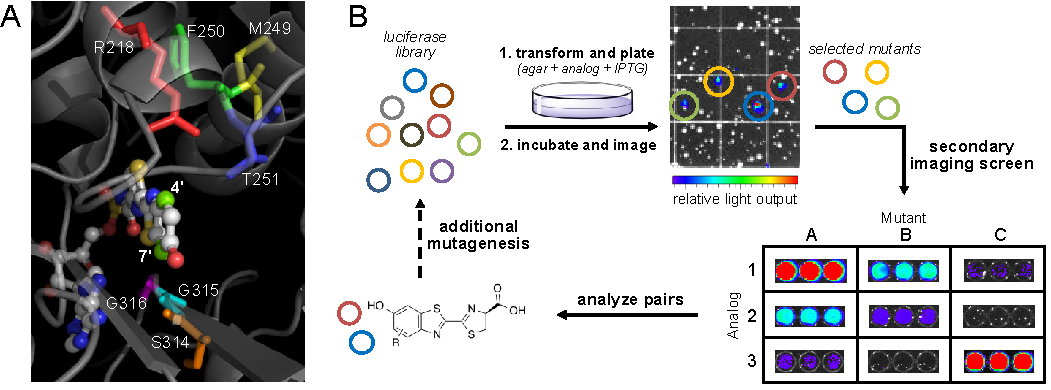
\includegraphics[width= \textwidth]{chapter2/fig3}
\centering
\caption[Generating mutant luciferase libraries and screening for orthogonal pairs]{Generating mutant luciferase libraries and screening for orthogonal pairs. (A) Amino acids targeted for mutagenesis. These residues were
selected based on their proximity to the 4′ and 7′ positions of luciferin. (B) Library screening strategy. An initial on-plate screen identified functional
mutants. These “hits” were subjected to a secondary screen for orthogonality with other mutants and luciferin analogues.}
  \label{fig:residues_screening}
\end{figure}
These selections were partially based on phylogenetic data gathered from across the insect luciferase
family,13,61 along with previous biochemical assays: Arg218 is
known to interact with \dluciferin{} and influence the local
structure of the binding pocket;29 F250 lies in close proximity
(∼3 Å) to the benzothiazole ring of \dluciferin{}; T251 has been
shown to potentiate substrate binding;30 residues 314−316 line
a critical edge near the luciferin phenolate and C7′ position.
Mutations at all of these target sites have been shown to perturb \dluciferin{} binding (and thus light emission), while
preserving the overall structural integrity of the enzyme.9,30,62
Saturation mutagenesis was used to prepare the desired
libraries. The degree of mutation applied at each residue was
based on the following considerations: sequence conservation
among the insect luciferase family, the identity of the native
residue, and the location of the residue. For example,
nonconserved residues were mutated to a higher degree
compared to conserved residues in the active site. Codon
compression methods were further used to eliminate
redundancies and reduce the number of transformants (Tables
S1 and S2).63 The final libraries ranged from 19 to 4800
members in size and were constructed using synthetic gene
assembly64 in combination with circular polymerase extension
cloning (CPEC) (Tables S3−S9).65
The libraries were screened for orthogonal substrate usage
using a two-tiered approach. Library DNA was first introduced
into bacteria, and the transformants were arrayed across agar
plates containing embedded luciferins (Figure \ref{fig:residues_screening}B). Light-emitting
colonies were easily identified, and in
some cases, the light emission values were on par with native
Fluc and \dluciferin{}. A handful of the
corresponding mutants were sequenced. Some mutations
were observed for multiple analogues, suggesting that they
might be selective for bulky luciferins. Other
mutations were unique to each compound, which is notable,
given the subtle structural differences between some of the
analogues. The number of colonies screened was ∼3× the
calculated diversity for each library.
While initial screens revealed functional mutants (and
quickly culled nonfunctional enzymes), they did not report
on selective substrate usage (i.e., orthogonality). The on-plate
screens also did not control overall expression levels and
differences in compound transport. To address these
parameters, we performed a secondary screen. Colonies
emitting detectable levels of light on-plate were selected and
expanded overnight. These cultures were then lysed and
imaged with analogues. Mutants that provided light emission
on par with native Fluc were identified as bona fide “hits” and
used to create next-generation sequences. This iterative process
was performed to evolve large pools of diverse, but functional,
enzymes. “Hits” from these subsequent generations were
ultimately tested with all luciferin analogues in secondary
screens.
To mine the entire collection of imaging data for substrateselective
pairs, we first developed a measure of orthogonality
(equation shown in Figure \ref{fig:mining_verifying}A).
\begin{figure}[htbp]
\includegraphics[width= \textwidth]{chapter2/fig4}
\centering
\caption[Analyzing orthogonal enzyme−substrate pairs]{Analyzing orthogonal enzyme−substrate pairs. (A) Representative emission of luciferase mutants screened against a panel of luciferin
analogues. These data were analyzed with a computer algorithm to determine lead mutants with the strongest orthogonality. (B) Purified mutants
exhibit orthogonality. Enzyme (1 μg) was incubated with 100 μM of luciferin analogues, and emission intensities were used to determine the
orthogonality quotient (the ratio of the total flux for the C4/C7 or C7/C4 pairings). The geometric mean is plotted, and the error bars represent the
95\% confidence intervals for n > 4 experiments. (C) Total flux for lead mutants B and C highlights substrate selectivity between C4′ and C7′
sterically modified luciferins. Error bars represent the standard error of the mean for n > 4 experiments.}
  \label{fig:mining_verifying}
\end{figure}
Favorable values are obtained
when two mutants (e.g., A and B) react robustly with unique
substrates (e.g., compounds 1 and 2, respectively) in a mutually
exclusive manner. Thus, the more selective a pair of enzymes
for their cognate substrates, the larger the orthogonality rating.
Since the number of potential pairings exceeded 3000 in our
data set, we wrote a computer script to rapidly examine all pairs
in an unbiased fashion. The program iterated through each
possible combination, calculating the corresponding orthogonality
rating. The script ultimately returned a list of pairs ranked
by their potential for orthogonality (and thus utility for
multicomponent imaging).
The top pairs identified by the script exhibited selectivity for
analogues 3b (mutants A and B) and 2b−d (mutant C). The
magnitude of each mutant’s preferencedefined as the
orthogonality quotientwas analyzed. As shown in Figure
\ref{fig:mining_verifying}B and C, mutants A and B exhibited nearly a 100-fold preference for 3b over other analogues, while mutant C strongly favored C7′-modified analogues. Similar trends in orthogonal substrate
usage were observed using bacterial lysates (Figure S9) and
across a range of luciferin concentrations (Figures S10 and
S11). Biochemical analyses further indicated that the “brightest”
mutant enzymes were those capable of most efficient substrate
turnover (Table \ref{tb:kinetics}).
\begin{table}
  \caption{Biochemical analyses of orthogonal enzyme−
substrate pairs}
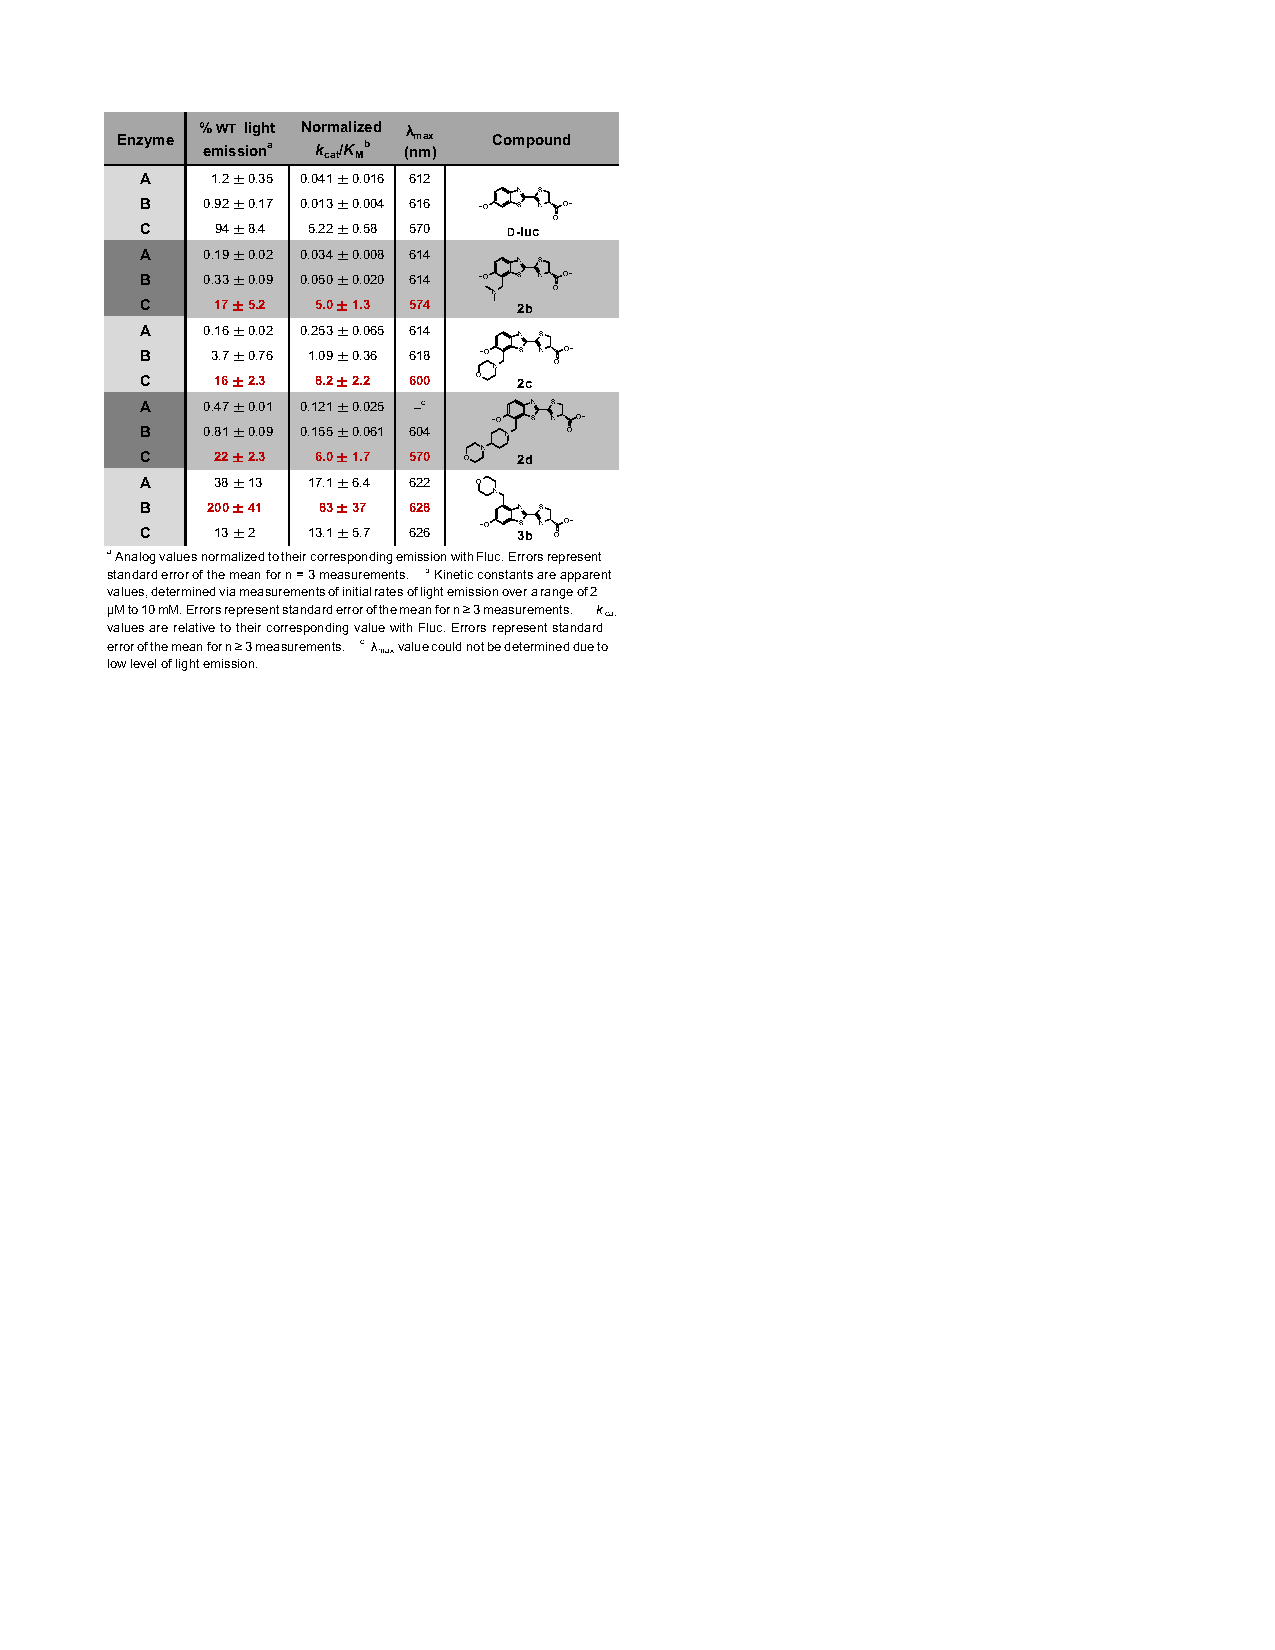
\includegraphics{chapter2/table1}
\centering
  \label{tb:kinetics}
\end{table}

\subsection*{Analyzing the origins of orthogonality}

The identities
of the mutant “hits” provided some insights into the origins of
substrate orthogonality. Mutant A had a single arginine to
alanine mutation at amino acid 218. Mutant B comprised the
same R218A mutation but harbored additional mutations at
residues 250 (Phe to Met), 314 (Ser to Thr), and 316 (Gly to
Thr). These residues are known to play a role in modulating
binding and interaction with the luciferin substrate. The R218A
mutant is especially interesting, as it is known to greatly reduce
light production and red shift emission with \dluciferin{}.29 It has
been hypothesized that the smaller Ala group allows more
water molecules to access the active site, potentially quenching
light emission.29 The bulky morpholino substituent of 3b could
fill this active site void to retain photon production. The third
mutant (mutant C) was more selective for the C7′-modified
luciferins compared to the C4′-modified compound. Mutant C
harbored a single mutation, R218K. R218K may slightly enlarge
the active site of the luciferase. This mutation has also been
shown to boost activity with bulkier cyclic aminoluciferin
analogues.22 The improved selectivity with 2b−d could be the
result of active site positioning. The C7′ substituents could
potentially place the luminophore in a more advantageous spot
for light emission.

To delve into the origins of selectivity, we prepared a small
library of additional mutants based on enzyme B (R218A,
F250M, S314T, G316T). R218A seemed critical for discriminating
the regioisomeric compounds, so this residue was held
constant across the series. All possible combinations of the
remaining mutations (F250M, S314T, G316T, or native Fluc
residues) were then allowed. Imaging analyses of these
combinatorial mutants indicated that R218A and F250M
were critical for luciferin discrimination (Figures S12 and
S13). Both mutations should result in a larger active site, but
why they preferentially accommodate 3b over other analogues
remains unknown. It is possible that the mutations disrupt
critical binding interactions with the luciferin core, but that
steric appendages (e.g., on the C4′ side) retain sufficient
contacts for subsequent oxidation. Indeed, when 3b was
incubated with R218A/F250M, light emission was maintained
(as compared to Fluc, Figure S13C). When \dluciferin{} and the
C7′-modified analogues were incubated with this same mutant,
though, light emission was drastically reduced. Interestingly, the
R218A/S314T mutant exhibited an opposite trend in analogue
selectivity: 2b was preferred to 3b (Figure S13C). Collectively,
these results suggest that mutant luciferases can be tuned to
respond to unique substrates. It is also possible that enzyme
orthogonality is most readily achieved not by improving the
utilization of one substrate but by diminishing reactivity with all
other substrates.

\subsection*{Cellular imaging with orthogonal pairs}

As a step
toward multicomponent imaging applications, we evaluated the
orthogonal enzymes and probes in cultured cell models.
Mammalian cell lines (HEK293 and DB7) were engineered
to express orthogonal mutants A−C. Equivalent expression
levels were confirmed using flow cytometry (Figure S14). Cells
were then incubated with analogues 2b−d and 3b, and photon
outputs were measured. As shown in Figure \ref{fig:in_vitro}, the substrates
were able to cross cell membranes and access the relevant
luciferases, resulting in sustained emission.
\begin{figure}[htbp]
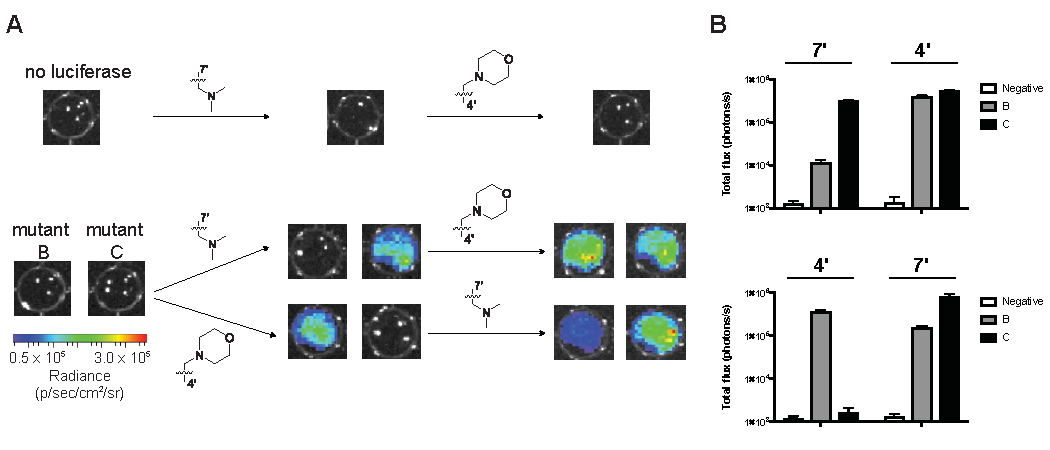
\includegraphics[width= \textwidth]{chapter2/fig5}
\centering
\caption[Imaging cells with orthogonal luciferase−luciferin pairs]{Imaging cells with orthogonal luciferase−luciferin pairs. (A) Mutant luciferase-expressing DB7 cells were plated (1.5 × 105 cells/well) in
96-well black plates and sequentially incubated with C4′ and C7′ sterically modified luciferins (750 μM). Representative bioluminescence images are
shown. (B) Quantification of the images from (A) after initial substrate addition. Error bars represent the standard error of the mean for experiments
performed in triplicate.}
  \label{fig:in_vitro}
\end{figure}
Photon production
was also confined to cells expressing the complementary
luciferase for each orthogonal luciferin: cells with mutant B
were only visible upon treatment with analogue 3b, whereas
cells with mutant C were only visible upon treatment with analogues 2b−d (Figures S15−S18). Importantly, the
orthogonal pairs could also distinguish unique cell types in a
single imaging session. For example, DB7 cells stably expressing
mutant B or C could be readily detected via sequential
administration of the requisite substrates (Figure 5). Similar
trends were observed upon imaging HEK293 cells (Figure S19)
and cocultures (Figure S20). These data suggest that crossreactivity
between mutants B and C and their non-orthogonal
substrates is minimal. The orthogonal pairs also exhibit unique
emission spectra (Figure S21) that can further enhance some
multicomponent imaging applications (Figure S22).

\section{Conclusions}

We developed a general strategy to evolve and identify mutant
versions of firefly luciferase that accept distinct, chemically
modified luciferins. Bioluminescence has been largely limited to
visualizing one biological feature at a time, as the most
advantageous luciferases and luciferins for whole-animal
imaging utilize the same substrate and cannot be distinguished
in vivo. To address this void, we generated a family of sterically
modified luciferins that were poor substrates for firefly
luciferase but inherently capable of producing light. Using an
on-plate screen, mutant versions of luciferase were identified
that could also catalyze light emission with other analogues.
Pools of these functional mutants were then further mined for
orthogonal pairs. Some of the mutants could selectively process
individual luciferins both in vitro and in cells, setting the stage
for multicomponent in vivo imaging.
Future studies will be aimed at generating additional
bioluminescent probes with improved brightness and other
optical properties. The enzyme−substrate “hits” reported here,
while immediately useful, are weaker light emitters than native
bioluminescent systems. Improved light outputs can be
achieved using additional rounds of mutagenesis and screening.
Previous studies have also demonstrated that distant mutations
can profoundly influence the architecture of the luciferase active
site, and these regions will be incorporated into future libraries.
The screening strategy is also broadly applicable to diverse
luciferins, including analogues with altered chromophores that
could provide drastically different colors of light. Our results suggest that enzymes capable of discriminating even subtle
substrate modifications can be readily identified. Such an
outcome bodes well for generating additional orthogonal pairs
and filling a long-standing void in imaging capabilities. We
anticipate that collections of designer luciferins and luciferases
will inspire new discoveries in a variety of disciplines, similar to
how fluorescent protein technology enabled seminal advancements
in numerous fields.

\bibliographystyle{achemso}
\bibliography{thesis, ch2}

%%% Local Variables: ***
%%% mode: latex ***
%%% TeX-master: "thesis.tex" ***
%%% End: ***

% !TEX root = ./thesis.tex

\chapter{Parallel Screening for Rapid Identification of Orthogonal Bioluminescent Tools}
\section{Introduction}
Our understanding of living systems is profoundly shaped by our ability to see biology in action. Central to these efforts are robust and translatable imaging tools.\cite{Specht:2017et,Lavis:2014jx}(1, 2) Decades of work to engineer and optimize fluorescent proteins have provided a palette of designer probes for cellular studies. Using combinations of these tools, it is now possible to trace the orchestrated behaviors of immune cells,\cite{Germain:2012ip}(3) nerve cell connections,\cite{Cai:2013dy}(4) and other interactions.\cite{Porterfield:2015bu}(5) Widespread application of fluorescent probes will continue to reveal unanticipated facets of biology. Concurrently, gaps in our knowledge will spur the development of innovative tools. Fluorescent probes endowed with novel functions (altered colors, photoswitches, etc.) are already enabling new pursuits.\cite{Rodriguez:2017ju,Betzig:2006hx}(6, 7)
\par
Biological discoveries will be further bolstered by advances in bioluminescent probe development. Bioluminescence relies on light generation via luciferase enzymes and luciferin small molecules.\cite{Prescher:2010dv,Branchini:2015epa}(8, 9) Since no excitation light is required, this modality is attractive for studies involving large length or time scales.\cite{Zhao:2005if,Rumyantsev:2016fd,Troy:2004bda}(10-12) Indeed, firefly luciferase (Fluc) and its cognate substrate (d-luciferin) are ubiquitously used in rodent models to interrogate molecular and cellular events.\cite{Adams:2014jsb,Xu:2016et}(13, 14) Fluc and its homologues have been further engineered to provide different colors of light.\cite{Branchini:2007fz,Nakatsu:2006esa}(15, 16) Such tools have been applied for multicomponent imaging in vitro. The wavelengths achieved, though, are unsatisfactory for routine use in vivo. Multicomponent imaging with even the most spectrally resolved probes remains challenging due to interference from surrounding tissue.\cite{Zhao:2005if}(10) As a consequence, bioluminescence has lagged behind fluorescence for multicellular studies in tissues and whole organisms.
\par
To realize multicomponent imaging in vivo, we turned to a more tractable parameter: substrate selectivity. Enzymes exhibiting mutually exclusive (i.e., orthogonal) substrate preferences should be readily distinguished in a variety of biological models. Fluc is remarkably tolerant of a variety of luciferin modifications, including both electronic\cite{Woodroofe:2012vx,McCutcheon:2012ixb,Conley:2012gha,Kuchimaru:2016eba}(17-21) and steric\cite{Steinhardt:2016in,Jones:2017be,Jathoul:2014do,Woodroofe:2008faa,Mofford:2014iwa}(22-26) derivatives. While dozens of luciferin analogues have been crafted, most result in reduced photon outputs relative to d-luciferin, the native substrate, at saturating doses.\cite{Rathbun:2017kj}(27) In some cases, boosts in light emission have been achieved using modified versions of the enzyme.\cite{Mofford:2014iwa,Jones:2017be}(23, 25) These results set the stage for developing designer luciferase?luciferin pairs, but few methods to systematically generate orthogonal sets have been pursued.\cite{Jones:2017be,Nishihara:2017bd}(25, 28) Substrate-selective luciferases are found in nature, and a handful have been coopted for dual imaging (e.g., combinations of d-luciferin- and coelenterazine-utilizing enzymes).(29-32) However, most remain suboptimal for use in vivo. The characterization of % TODO continue here
other naturally occurring luciferases and luciferins has also not kept pace with the demand for new pairs. Consequently, bioluminescence imaging has been limited by a lack of mutually orthogonal enzymes and substrates.
\par
We aimed to expedite the search for luciferases that exhibit unique preferences for distinct luciferin analogues. Accessing enzymes with alternative substrate use is well precedented in directed evolution.(33-35) However, traditional applications of this technique have focused on optimizing one enzyme at a time. Selectivity for one molecule over another is often realized as a consequence, but is not typically the parameter being screened.(36-41) Here, we present a general and rapid approach to achieve substrate selectivity and engineer orthogonal luciferase?luciferin pairs. This strategy relies on parallel screening of functional luciferases with collections of chemically diverse luciferins (Figure 1a). The large data sets are then mined for orthogonal combinations using a custom computer script. Enzyme?substrate pairs are deemed orthogonal if robust reactivity is observed when complementary partners interact, but minimal to no reactivity is observed in all other cases (Figure 1a). Collectively, we screened 159 mutants and 12 analogues, generating a candidate list of greater than 800,000 possible pairs. We evaluated the orthogonality of 175 pairs in vitro. A subset was successfully applied in cultured cell and animal models, highlighting the feasibility and translatability of the approach. We also analyzed principles governing selective substrate use and identified methods to search for expanded collections of orthogonal imaging agents. Overall, this work greatly expands the number of viable bioluminescence probes for multicomponent imaging and presents a strategy to accelerate the identification of new ones. The parallel screening method is also applicable to other areas where selective substrate use is required.

\section{Results and discussion}
\subsection*{Expanding the Pool of Candidate Luciferins and Luciferases}
As a starting point for substrate modification, we focused on d-luciferin derivatives with steric appendages at C4? and C7?. These positions lie in close proximity to the Fluc backbone,(42) and preliminary work revealed that modifications here do not quench or otherwise impede photon emission.(25) We also previously identified a pair of luciferases that could discriminate between luciferins with modifications at these positions,(25) suggesting that they were good starting points for new probe development. However, attempts to optimize this pair via traditional directed evolution (focusing on one enzyme at a time) did not result in improved substrate selectivity (Figure S1).
\par
We reasoned that screening for selectivity at the outset would provide a more rapid route to new bioluminescent pairs. Engineering luciferases to discriminate among structurally similar compounds can be difficult.(23, 43) Thus, we initially focused on diversifying the enzyme and substrate inputs. Collections of both new and known(24, 25) luciferins were assembled (Figure 1b). These molecules covered a broad range of chemical space and comprised both hydrophilic and hydrophobic functional groups. The luciferins were benchmarked for light emission with Fluc (Figure S2). All compounds were functional light emitters, though they varied in terms of photon output. Some level of enzyme activity is necessary for successful evolution, but weak performers can be advantageous starting points for evolving new functions.(33)
\par
In parallel with luciferin diversification, we targeted broad sectors of Fluc sequence space for mutagenesis. Twenty-three residues near the active site were selected, and the mutations were covered in 8 libraries (labeled in Figure 1c). The majority of the mutants would likely be nonfunctional, and thus not ideal starting points for probe development. We aimed to eliminate these luciferases early on and perform parallel screens with an enriched pool of viable mutants. Such an approach would save time and reagents as luciferases are not amenable to high-volume separations (e.g., FACS) or selections; rather, each mutant must be physically interrogated with a given substrate. We adapted a high-throughput method to traverse the luciferase libraries and cull nonfunctional members (Figure S3a).(25) The libraries were transformed into bacteria, and the transformants were grown on agar containing one of four minimally perturbed luciferins: 4?/7?-BrLuc or 4?/7?-MeLuc (Figure 1b, Figure S3a). These analogues were selected for on-plate screens since they are among the ?brightest? emitters and easy to access in bulk. Light-emitting colonies were picked and further assayed in lysate and by sequencing (Figure S3a). A variety of mutants were identified (Figure S4), including enzymes that were unique to each luciferin. Some hits were further diversified (1?3 generations) via random mutagenesis to enlarge the pool of luciferase mutants (Table S1 and Figure S3).

\subsection*{Screening for Orthogonal Luciferase?Luciferin Pairs in Silico}
With enriched sets of functional luciferases, we aimed to screen the collection for orthogonal pairs. Testing each combination of two mutants and two substrates would have required 829,026 separate experiments (Figure 2a), an impractical number. Instead, we screened each analogue across the same panel of 159 luciferases, generating 1908 (12 substrates x 159 enzymes) individual data points (Figure S3b). An ideal orthogonal enzyme would be ?positively? matched with a single substrate and ?negatively? matched with all other luciferins. To identify such enzymes, we established a metric to quantify orthogonality and mine the data. We reasoned that perfect selectivity could be represented by an identity matrix (Figure S5, Supplementary Note). Orthogonality would be maximal if each enzyme was completely selective for its cognate substrate (represented by a ?1? in the identity matrix) and nonfunctional with other luciferins (?0? in the identity matrix). An orthogonality score was determined by representing each set of two luciferases and two luciferins as a square matrix, with enzymes in rows and substrates in columns. These data were compared to the ideal case (identity matrix) via root-mean-square distance (RMSD). The RMSD values were then converted to numeric values (i.e., orthogonality scores) representing the fold resolution between the positive and negative pairings (see Supplementary Note for more details). We wrote a computer script to assemble each possible matrix from the screening data and calculate the orthogonality of each pairing. The pairs were sorted by increasing RMSD, with the smallest value (highest orthogonality score) representing the most orthogonal pair.
\par
The algorithm provided a ranked list of the 829,026 possible orthogonal sets (Figure 2a). The top pair comprised analogues 2 and 11 (4?-MorphoLuc and 7?-MorPipLuc) with mutants 81 and 104 (Figure 2a). Selective light emission with these enzymes and substrates was verified in vitro (Figure 2b). We further validated the top ten unique pairings on the ranked list, along with a handful of others in the data set (every tenth rank among the top 100, every 100th rank among the top 1000, and every 1000th rank down to position 5000). In all cases, orthogonality scores were measured in bacterial lysate (Figure 2c). Among the top 1000 pairs, >10-fold photon outputs were observed with the positively paired luciferase?luciferin set compared to the negatively paired set (Figure 2c). Diminishments in selectivity were observed farther down the list. These results suggest that the in silico rank order is a good predictor of orthogonal substrate use. The method also culled 99.9\% (?828,000 of the total 829,026) of irrelevant enzyme?substrate pairings (Figure S6), enabling fast convergence on important hits. As more luciferases and luciferins are screened, the data set can be expanded and continually mined for new orthogonal pairs.

\subsection*{Imaging with Orthogonal Pairs in Cultured Cell and Animal Models}
We aimed to transition lead pairs from the screening analyses to mammalian cell imaging. In these more complex environments, issues of enzyme stability, substrate biocompatibility, and compound transport are of paramount concern. Fortunately, our approach to enriching functional luciferases preselects for luciferases and luciferins that are well behaved. Three of the top pairs from the script were analyzed in cultured cell (Figure S7) and animal models (Figure 3): (1) 4?-MorphoLuc/enzyme 81 (R218A, F250M, S314T, G316T) with 7?-DMAMeLuc/enzyme 37 (R218K), (2) 7?-MeLuc/enzyme 87 (R218K, F250Y, S314T, G316T) with 4?-BrLuc/enzyme 53 (V240I, V241M, F243M, F247Y, S347G), and (3) 4?-BrLuc/enzyme 51 (F243M, S347G) with d-luciferin/enzyme 93 (R218K, M249L, S314T, G316S). These pairs were selected due to the ease of accessing the substrates, along with their relative brightness. The mutants were stably expressed in DB7 mouse mammary carcinoma cells. The cells were treated with relevant luciferins and imaged (Figure S7). Substrate specificity was maintained in all cases, highlighting the success of the parallel screening method.
\par
Selectivity was also maintained in vivo. DB7 cells expressing the relevant mutants were implanted in FVB/NJ mice. Subsequent administration of the complementary luciferin analogues resulted in light emission for positively paired compounds with minimal cross reactivity (Figure 3). These images mark an initial demonstration of dual imaging with purely engineered luciferase?luciferin pairs. It is also important to note that perfect resolution is not required for multicomponent imaging applications. Rather, patterns of substrate use can serve as diagnostic fingerprints.(44) Photon outputs from the orthogonal pairs are in a useful range for monitoring bulk cell populations. The dimmest set (enzyme 37/7?-DMAMeLuc and enzyme 81/4?-MorphoLuc) emits enough photons to visualize ?6 x 106 cells in subcutaneous models. The other orthogonal sets are substantially brighter and can enable more sensitive imaging. Collectively, these data show that parallel screens and in silico analyses can be used to identify and transition orthogonal sets to a variety of biological models.

\subsection*{Analyzing Trends in Orthogonal Substrate Use}
To gain insight into principles governing orthogonality, we undertook a detailed analysis of the screening results. The highest-ranked pairs comprised a variety of enzymes and substrates. Seven unique luciferins (from both the 4? and 7? series) were found among the top 10 pairs, along with luciferases comprising mutations at 18 unique sites (Supplementary Data; Figure S8). The diversity in hits implies that there are a variety of paths to achieve substrate resolution. Among the pairs, orthogonality was primarily realized not by markedly enhanced turnover of a preferred substrate. Rather, selectivity arose from reduced photon production with other compounds. As shown in Figure 4a, matched enzymes and substrates (positive pairs) were on par with native Fluc in terms of photon output. The unmatched enzymes and substrates (negative pairs), by contrast, demonstrated reduced activities (?10?1000-fold lower). Thus, in a given orthogonal pair, selectivity is mostly achieved by reducing light emission with the negatively paired compound versus selectively increasing light emission with the positively paired compound. For example, mutant 81 provides ?4-fold enhanced light output with 4?-MorphoLuc compared to Fluc. With every other luciferin screened, including the negatively paired compound 7?-MorPipLuc, mutant 81 emits >10-fold fewer photons than the native enzyme. So while light output with 4?-MorphoLuc is slightly improved with mutant 81, the decrease in light emission observed with 7?-MorPipLuc (>100-fold) contributes more to orthogonality.
\par
Since compound selectivity appears to be achieved by destroying enzyme?substrate interactions, structurally related compounds would be expected to exhibit similar trends in orthogonality. Indeed, bulky 7?-modified compounds tend to positively pair with the same types of enzymes (Figure S9). Many of these mutants (e.g., mutant 104) likely harbor space in the active site to accommodate 7? substituents (Figure S9a). Conversely, 4?-modified luciferins tend to produce less light with these same mutants and are thus negatively paired. Structurally divergent compounds were also more likely to comprise an orthogonal pair (Figure 4b). For example, substrates with a modification at the 4? position were rarely orthogonal to other 4? compounds. It is probably difficult to destroy activity with one 4?-modified compound without impacting others in the same series. When 4?- and 7?-modified substrates are paired, though, each substrate likely interacts differently with the enzyme, making it easier to achieve orthogonality. These results suggest a strategy for continued orthogonal bioluminescent probe development: incorporate more diverse analogues in parallel screens.
\par
Some compounds appear uniquely suited for orthogonal probe development. For example, 4?-BrLuc shows up nearly twice as often in the top 1,000 hits compared to other compounds (Figure S10). The mechanistic basis for this preference is unclear. The bromine substituent is roughly the same size as the methyl group in 4?-MeLuc, negating a pure steric argument. 4?-MeOHLuc is predicted to form orthogonal pairs (albeit less frequently) with similar compounds as 4?-BrLuc (Figure 4), suggesting that polarizable substituents might be preferred. Heavy halogen atoms (e.g., Br) are also known to quench the fluorescence of some molecules via intersystem crossing.(45) Thus, certain 4?-BrLuc conformations could result in internal quenching (and poor light emission) and thus pair negatively with several mutants. Additional compound screens and analyses will be necessary to discriminate among these possibilities and gain more insight.
\par
We further analyzed the frequency of positive and negative pairings between luciferins and individual residues (Figure 5). Luciferases with mutations at residues 240, 247, or 347 seemed to prefer 4?-modified compounds. These residues are known to modulate the binding and light emission of the native substrate, d-luciferin.(43, 46-48) Docking studies corroborated these findings, suggesting that the mutations (e.g., S347G in mutants 51 and 53) likely create space for bulky substituents (e.g., 4?-BrLuc, Figure S11). These residues are also negatively paired with most of the 7?-modified compounds, suggesting that they are good candidates for future orthogonal probe design. Surprisingly few hot spot residues correlated with selective 7? analogue use (Figure 5). Fluc residues near C7? primarily comprise backbone amides.(42, 49) Thus, it is unclear how specificity for these analogues might arise.

\subsection*{Added Diversity Improves Orthogonality}
Multicomponent imaging requires not just pairs of orthogonal enzymes and substrates, but also triplets, quadruplets, and higher order sets. Identifying such expanded collections requires structurally diverse enzyme and substrate architectures. If only a few privileged luciferases or luciferins from our data set could provide the desired selectivities, it would be difficult to achieve larger collections of orthogonal probes. To assess whether we were approaching an upper limit on orthogonality, we performed simulations within the existing data set. Random subsets of various sizes were selected from the full pool of substrates and enzymes. The sets were analyzed using the algorithm from above, and orthogonality scores were generated (Figure 6a). Regardless of the identities of enzymes or substrates used, scores increased with greater numbers of both enzymes (from 2 to 159) and substrates (from 2 to 12). This result implies that we have not reached a plateau in identifying orthogonal pairs. Exploring more sequence space with mutant luciferases and chemical space with modified luciferins should also improve the orthogonality of the top pairings.
\par
As a next step, we modified the algorithm to search for not just two pairs of orthogonal probes but also triplets and multiple sets in general. A set of three adds significant complexity, as not only three positive pairings, but also six negative pairings, must be identified. From our current data set, this required sifting through >144 million combinations. We combed the original data set in search of three mutually orthogonal enzyme?substrate pairs. A total of 6171 potential sets were identified. The orthogonalities of the top ten were verified in bacterial lysate (Figure S11). The top triplet set is shown in Figure 6b and comprises two enzyme?substrate pairs previously validated in vivo. The overall orthogonality score for this set was lower than that of the individual pairs from above. However, this result represents key proof-of-concept and a starting point for the development of larger collections of mutually orthogonal luciferase?luciferin sets. Perfect selectivity is also not required for using the probes in biological environments. Rather, patterns in substrate use are most important and can be discerned using standard imaging equipment and rates of change in photon output.

\section{Conclusions}
We developed a general and rapid strategy to engineer orthogonal luciferase?luciferin pairs. The method relies on developing an initial pool of functional enzymes and screening the collection with chemically diverse luciferins. Using this approach, we generated >800,000 possible pairings and mined the data for orthogonal pairs with a custom computer algorithm. Dozens of candidates were identified and validated in vitro. A handful of hits were further translated into cultured cell and animal models, greatly expanding the number of bioluminescent probes for multicomponent imaging.
\par
We further analyzed the principles governing orthogonal substrate use. Chemical and sequence diversity was key to eliciting high levels of selectivity. Thus, the addition of more luciferins and libraries to our ?living? data set should improve orthogonality and lower the barrier to identifying higher-order sets. A fleet of sensitive, selective pairs will bolster imaging capabilities and push the boundaries of what we can ?see? and learn about biological systems. The methods reported here are also applicable beyond the field of bioluminescence. Parallel screens and in silico analyses can expedite the search for other orthogonal enzyme?substrate or protein?ligand pairs relevant to optogenetics, cell signaling, and other disciplines.

\bibliographystyle{achemso}
\bibliography{thesis2}

%%% Local Variables: ***
%%% mode: latex ***
%%% TeX-master: "thesis.tex" ***
%%% End: ***
\chapter{Multicomponent bioluminescence imaging via substrate unmixing}
\section{Introduction}
\section{Results and Discussion}
\subsection*{title}
\section{Conclusions}

\bibliographystyle{achemso}
\bibliography{thesis2}

%%% Local Variables: ***
%%% mode: latex ***
%%% TeX-master: "thesis.tex" ***
%%% End: ***

% ... and so on

% These commands fix an odd problem in which the bibliography line
% of the Table of Contents shows the wrong page number.
\clearpage
\phantomsection

% "References should be formatted in style most common in discipline",
% abbrv is only a suggestion. Comment out if formatting for a bib after each chapter.
%\bibliographystyle{achemso}
%\bibliography{thesis2}

% The Thesis Manual says not to include appendix figures and tables in
% the List of Figures and Tables, respectively, so these commands from
% the caption package turn it off from this point onwards. If needed,
% it can be re-enabled later (using list=yes argument).
\captionsetup[figure]{list=no}
\captionsetup[table]{list=no}

% If you have an appendix, it should come after the references.
% The original template (from Trevor) had a custom \appendix command,
% but I found it to break figure/table counters. I'm not sure how
% reliable my fix is, so I ended up reverting back to the standard
% latex version, and renaming the custom command to \myappendix.  You
% can try both and see how things work out:
% 1) Call \appendix once, and then make each appendix a \chapter
% 2) Call \myappendix once, and then make each appendix a \section.

\appendix
\chapter{Appendix Title}

Supplementary material goes here. See for instance Figure
\ref{fig:quote}.

\section{Lorem Ipsum}

dolor sit amet, consectetur adipisicing elit, sed do eiusmod tempor
incididunt ut labore et dolore magna aliqua. Ut enim ad minim veniam,
quis nostrud exercitation ullamco laboris nisi ut aliquip ex ea
commodo consequat. Duis aute irure dolor in reprehenderit in voluptate
velit esse cillum dolore eu fugiat nulla pariatur. Excepteur sint
occaecat cupidatat non proident, sunt in culpa qui officia deserunt
mollit anim id est laborum.

\begin{figure}
  \centering
  \begin{tabular}{l}
    ``I am glad I was up so late,\\
    \quad{}for that's the reason I was up so early.''\\
    \em \footnotesize William Shakespeare (1564-1616), British
    dramatist, poet.\\
    \em \footnotesize Cloten, in Cymbeline, act 2, sc. 3, l. 33-4.
  \end{tabular}
  \caption{A deep quote.}
  \label{fig:quote}
\end{figure}


%%% Local Variables: ***
%%% mode: latex ***
%%% TeX-master: "thesis.tex" ***
%%% End: ***


\end{document}
